\documentclass[brudnopis]{xmgr}
% Jeśli nowe rozdziały mają się zaczynać na stronach
% nieparzystych:
%\documentclass[openright]{xmgr}

%\defaultfontfeatures{Scale=MatchLowercase}
%\setmainfont[Numbers=OldStyle,Ligatures=TeX]{Minion Pro}
%\setsansfont[Numbers=OldStyle,Ligatures=TeX]{Myriad Pro}
% for fontspec version < 2.0
\setmainfont[Numbers=OldStyle,Mapping=tex-text]{Minion Pro}
\setsansfont[Numbers=OldStyle,Mapping=tex-text]{Myriad Pro}
%\setmonofont[Scale=0.75]{Monaco}

% Opcjonalnie identyfikator dokumentu
% drukowany tylko z włączoną opcją 'brudnopis':
\wersja   {wersja wstępna [\ymdtoday]}

\author   {Kamil Pek}
\nralbumu {231\,050}
\email    {kpek@sigma.ug.edu.pl}

\title    {TrainCMS --- System zarządzania treścią witryny internetowej}
\date     {2017}
\miejsce  {Gdańsk}

\opiekun  {dr W. Bzyl}

% dodatkowe polecenia
%\renewcommand{\filename}[1]{\texttt{#1}}
%\definecolor{stress}{cmyk}{0,1,0.13,0} % RubineRed
%\definecolor{topic}{cmyk}{0.98,0.13,0,0.43} % MidnightBlue

\begin{document}

% streszczenie
\begin{abstract}
W pracy przedstawiono wersję beta systemu zarządzania treścią witryny internetowej „TrainCMS”. W trakcie pracy zaimplementowano publikowanie artykułów, kategoryzację, wyświetlanie listy kategorii na pasku nawigacji. Stworzono User Interface, który wyświetla wszystkie artykuły na stronie głównej, niezależnie od kategorii w kolejności malejącej od daty dodania oraz kalendarz wydarzeń. Do artykułów i wydarzeń w kalendarzu zaimplementowano możliwość załączania ilustracji oraz dodawania komentarzy.

Zaimplementowano panel administratora do zarządzania artykułami, kategoriami, komentarzami, tagami, użytkownikami i kalendarzem oraz do podglądu statystyk.

Do implementacji użyto technologie takie jak Ruby, Ruby on Rails, ZURB Foundation, jQuery Turbolinks, Plataformatec Devise, CarrierWave, RMagick, reCAPTCHA, CKEditor, Chartkick, Prawn.
\end{abstract}

% słowa kluczowe
\keywords{cms, ruby on rails, calendar, comments, tags}

% tytuł i spis treści
\maketitle

% wstęp
\introduction
Podczas kilkuletniej pracy z najpopularniejszymi aplikacjami w tej kategorii, takimi jak Joomla i WordPress nabyłem doświadczenie oraz swój pogląd na to jak ma wyglądać system zarządzania treścią (ang. Content Managment System, CMS). Naturalnym stało się więc stworzenie własnego systemu, przy okazji prezentując jak najszerszą część umiejętności nabytych w trakcie trwania studiów.

Istniejące systemy są często wybierane przez między innymi lokalne serwisy informacyjne, przedsiębiorstwa i instytucje, dlatego w swoim systemie zawarłem funkcjonalności, które na pewno przydadzą się różnym podmiotom w skutecznym zaistnieniu w Internecie.

Podczas tworzenia interfejsu użytkownika i administratora, kierowałem się głównie ergonomią użytkowania i przedstawieniem możliwości jakie prezentuje system w jak najbardziej przystępny sposób tak, aby początkujący użytkownik mógł poruszać się w sposób intuicyjny po aplikacji.

\chapter{Wstęp i opis problemu}

\section{Porównanie dostępnych rozwiązań}

Na rynku systemów zarządzania treścią znajdziemy sporo różnych rozwiązań. W~dalszej części rozdziału przybliżę dwa najbardziej popularne produkty, będzie to Joomla i WordPress. Systemy różnią się od siebie pod wieloma względami. Rozwiązanie przedstawione przeze mnie jakim jest TrainCMS różni się  przede wszystkim technologią wykonania, gdyż oba wcześniej wymienione systemy wyprodukowane są technologii języka PHP i bazy danych MySQL, gdzie mój system opiera się na frameworku Ruby On Rails i bazie danych PostgreSQL.

\subsection{Joomla!}

Joomla jest to system zarządzania treścią, napisany w języku PHP, wykorzystujący do swojego działania system zarządzania bazą danych MySQL, rozpowszechniany na licencji GPL i jest dostępny bezpłatnie. Nazwa Joomla w języku suahili oznacza razem.   
System ten oferuję obsługę wielu kont użytkownika, wyszukiwarkę zaimplementowaną w User Interface, tworzenie wydruków artykułów, dołączanie ilustracji do artykułu, komentowanie artykułów przez niezalogowanych użytkowników. Wymienione funkcjonalności pokrywają się z możliwościami stworzonego przeze mnie systemu. 

TrainCMS posiada także inne możliwości, których nie oferuję Joomla w wersji podstawowej, jest to kalendarz wydarzeń, dodawanie załączników, generowanie dokumentów pdf zawierających artykuły, przedstawienie statystyk w formie graficznej, karuzela ilustracji wyróżnionych artykułów. Natomiast niektóre z rozwiązań zostały rozszerzone względem Joomli są to komentarze, które w projekcie TrainCMS rejestrują adres IP komentującego. 

Znajdziemy także w Joomli takie funkcję, których nie posiada mój system. Jednym z takich rozwiązań jest tworzenie zagnieżdżonej struktury menu w formie drzewiastej. Kolejnym rozwiązaniem jest możliwość zmiany szablonu frontu strony i szablonu zaplecza witryny. Główną funkcjonalnością Joomli jest możliwość łatwego rozszerzania możliwości strony za pomocą pluginów i komponentów. Podczas porównywania obu systemów należy pamiętać, że Joomla jest produktem z wieloletnim doświadczeniem na rynku, tworzonym przez zespół programistów z całego świata. Rozwiązania oparte na Joomli znajdują zastosowanie głównie przy dużych witrynach.

\subsection{WordPress}

WordPress jest systemem zarządzania treścią napisanym w języku PHP, wykorzystujący systemem zarządzania bazą danych MySQL i jest dystrybuowany na licencji GPL i dostępny bezpłatnie. 

System WordPress jest zdecydowanie mniej rozbudowany w porównaniu do Joomli. Oferuje on takie funkcjonalności jak podstawową kategoryzację, tagowanie i komentowanie artykułów, obsługę wielu kont użytkownika, odrębny interfejs dla użytkownika gościa, zwykłego użytkownika i administratora oraz podgląd statystyk jest również w pełny responsywny. Wszystkie wymienione funkcjonalności pokrywają się z zaimplementowanymi w systemie TrainCMS.

W TrainCMS znajdziemy także inne możliwości, których nie oferuję WordPress w wersji podstawowej, jest to kalendarz wydarzeń, dodawanie załączników, generowanie dokumentów pdf zawierających artykuły oraz karuzela ilustracji wyróżnionych artykułów. Natomiast niektóre z rozwiązań zostały rozszerzone względem Joomli są to komentarze, które w projekcie TrainCMS rejestrują adres IP komentującego. 

Należy w tym miejscu wspomnieć, że główną funkcjonalnością WordPress jest łatwość instalacji i zmiany wielu dostępnych szablonów strony. WordPress jest produktem z utartą pozycja na rynku systemów zarządzania treścią, który podobnie jak Joomla jest tworzony przez zespół programistów z całego świata. Witryny obsługiwane przez WordPress to głównie blogi.

\newpage

\section{Możliwości zastosowania praktycznego}

System TrainCMS został opracowany w taki sposób, aby sprostać wielu wymaganiom różnych użytkowników. Oferuje sporo możliwości, które przypadną do gustu każdemu i będą zarazem bardzo przydatne w codziennej pracy nad własna witryną Internetową. Reasumując możliwości serwisu ogranicza jedynie wyobraźnia administratora.

\subsection{Strona wizytkówa}

W celu stworzenia optymalnej i efektownej strony wizytówki należałoby stworzyć dowolną, zależna od potrzeb ilość artykułów, które zawierać by mogły na przykład dane kontaktowe do firmy, kolejny artykuł zawierać by mógł referencję, natomiast kolejny parę zdań o firmie i jej profilu działalności. Po odpowiednim według operatora strony rozmieszczeniu informacji możemy przejść do podglądu statystyk, które w tym przypadku mogą wyświetlić informację na przykład o tym, która sekcji informacji jest najbardziej popularna. W tego rodzaju rozwiązaniu można by było się zastanowić na koniecznością włączenia modułu komentarzy. 

\subsection{Internetowe portfolio}

Każda osoba tworząca w internecie portfolio swojej działalności zamierza przyciągnąć tym samym jak największą liczbę nowy klientów. Aby skutecznie rozwiązać ten problem proponuję każde dzieło opisywać w osobnym artykule. Natomiast informację, którą klient zechciałyby umieścić na szczycie należy zaznaczyć atrybut wyróżniony.

\subsection{Serwis informacyjny}

W tym rozwiązaniu znajdą zastosowanie wszystkie zaimplementowane w systemie funkcjonalności. Większość rozwiązań została wyprofilowana właśnie na tego typu zastosowania. Głównym szkieletem w tym przypadku będzie możliwość tworzenia wielu kategorii, gdzie redaktor takiego serwisu będzie mógł z pełną łatwością organizować wszystkie tematy poruszane na portalu i jednocześnie wszystkie artykuły z każdej kategorii będą wyświetlane na stronie głównej. Gorące tematy będzie można oznaczać jako wyróżnione i tym sposobem będą przez cały widoczne na szczycie karuzeli. Gość odwiedzający serwis z łatwością wejdzie w interakcję poprzez system komentarzy, operator serwisu będzie mógł korzystać z przejrzystych statystyk i za ich pomocą wyciągać wnioski na temat pracy portalu i planować dalszy jego rozwój. Z pomocą dla nowych gości przyjdą tagi, dzięki którym będzie można szybko wyszukać artykuły poruszające dany temat. Łatwiejsze stanie się planowanie różnego rodzaju imprez za pomocą wbudowanego kalendarza wydarzeń. Autor piszący artykuły dla serwisu nie będzie musiał zagłębiać się w panel zaplecza, na stronie głównej po zalogowaniu znajdzie skróty do najpotrzebniejszych funkcjonalności takich jak nowy artykuł, lista swoich artykułów oraz lista komentarzy pod swoimi artykułami.

\chapter{Projekt i analiza}

\section{Diagram związków encji}

\begin{figure}[!tbh]
\centering
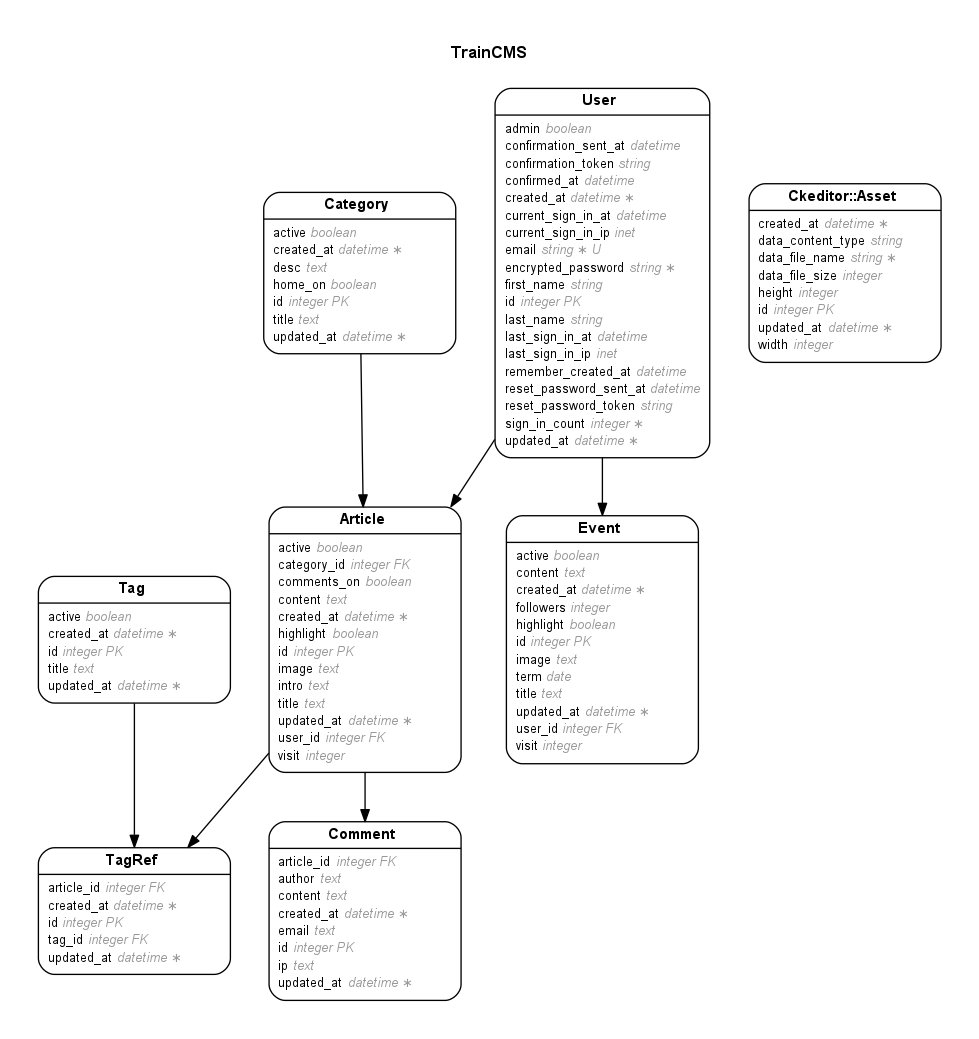
\includegraphics[width=.86\linewidth]{fig/erd}
\caption{Diagram związków encji\label{RYS.1}}
\source{Opracowanie własne}
\end{figure}

\section{Diagram modelu danych}
Diagram modelu danych

\section{Projekt interfejsu użytkownika}
Projekt GUI

\chapter{Implementacja}

\section{Architektura rozwiązania - Ruby on Rails}
ROR

\section{ZURB Foundation}
Foundation

\section{CarrierWave}
CarrierWave

\section{Prawn}
Prawn

\chapter{Bibliografia}

\section{ksiązki}
ebooks

\section{zasoby Internetu}
stackoverflow

\section{dokumentacja na GitHub.com}
git jest gitwbzyl semi

% zakończenie
\summary
Możliwości, jakie stoją przed archiwum prac magisterskich opartych na
XML-u, są ograniczone jedynie czasem, jaki należy poświęcić na pełną
implementację systemu. Nie ma przeszkód technologicznych do stworzenia
co najmniej równie doskonałego repozytorium, jak ma to miejsce w
przypadku ETD. Jeżeli chcemy w pełni uczestniczyć w rozwoju nowej ery
informacji, musimy szczególną uwagę przykładać do odpowiedniej
klasyfikacji i archiwizacji danych. Sądzę, że język XML znacznie to
upraszcza.

% załączniki (opcjonalnie):
\appendix
\chapter{Tytuł załącznika jeden}

Treść załącznika jeden.

\chapter{Tytuł załącznika dwa}

Treść załącznika dwa.

% literatura (obowiązkowo):
\bibliographystyle{unsrt}
\bibliography{xml}

% spis tabel (jeżeli jest potrzebny):
\listoftables

% spis rysunków (jeżeli jest potrzebny):
\listoffigures

\oswiadczenie

\end{document}
